\documentclass[11pt,aspectratio=169]{beamer}

% Packages
% Shared content style for NN and NNDS. Written by Claude (2026-10-14).
%
% Everything that shared slides rely on lives here, loaded by both courses:
% colors, notation helpers and the card system. Course themes own only the
% presentation around the content (header, footer, title page, fonts, the
% \myalert color and where \SlideSource text goes). Change a definition here,
% never by redefining it in a course file, so the two courses cannot drift.

\usepackage{mathtools,amssymb,tcolorbox}
\tcbsetforeverylayer{autoparskip}

% Semantic colors
\definecolor{darkred}{rgb}{0.55,0,0}
\definecolor{darkpastelblue}{rgb}{0.47,0.62,0.8}
\definecolor{darkcerulean}{rgb}{0.03,0.27,0.49}
\definecolor{darkgreen}{rgb}{0,0.55,0}

% Figure palette (draw.io defaults)
\definecolor{titlecolor}{RGB}{245, 242, 238}
\definecolor{drawgray}{HTML}{666666}
\definecolor{drawgray_l}{HTML}{F5F5F5}
\definecolor{drawblue}{HTML}{6C8EBF}
\definecolor{drawblue_l}{HTML}{DAE8FC}
\definecolor{drawgreen}{HTML}{82B366}
\definecolor{drawgreen_l}{HTML}{D5E8D4}
\definecolor{draworange}{HTML}{D79B00}
\definecolor{draworange_l}{HTML}{FFE6CC}
\definecolor{drawyellow}{HTML}{D6B656}
\definecolor{drawyellow_l}{HTML}{FFF2CC}
\definecolor{drawred}{HTML}{B85450}
\definecolor{drawred_l}{HTML}{EA6B66}
\definecolor{drawviolet}{HTML}{9673A6}
\definecolor{drawviolet_l}{HTML}{E1D5E7}

% Notation
\newcommand{\vc}[1]{\boldsymbol{\mathbf{#1}}}
\DeclareMathOperator*{\argmax}{arg\,max}
\DeclareMathOperator*{\argmin}{arg\,min}

% Cards: blue for definitions and computable quantities, green for goals and
% stable formulations, orange for warnings and trade-offs, red for
% training-specific or problematic elements.
\tcbset{
	nndsblue/.style={colback=drawblue_l!35!white,colframe=drawblue,boxrule=0.8pt,arc=1mm},
	nndsgreen/.style={colback=drawgreen_l!35!white,colframe=drawgreen,boxrule=0.8pt,arc=1mm},
	nndsorange/.style={colback=draworange_l!35!white,colframe=draworange,boxrule=0.8pt,arc=1mm},
	nndsred/.style={colback=drawred_l!12!white,colframe=drawred,boxrule=0.8pt,arc=1mm}
}

% A card that opens with \[ would start with an empty paragraph line plus the
% display skip, leaving more room above than below (by an amount that differs
% between engines). Set that leading equation as a centered display-style line
% instead, so the space above it is the card padding, as below.
\makeatletter
\newcommand{\nndscardlead}{\futurelet\nndscard@next\nndscard@check}
% tcolorbox follows this hook with \ignorespaces; look past it.
\def\nndscard@check{\ifx\nndscard@next\ignorespaces
	\expandafter\nndscard@skip\else\expandafter\nndscard@test\fi}
\def\nndscard@skip\ignorespaces{\nndscard@test}
\newcommand{\nndscard@test}{\@ifnextchar\[{\nndscard@display}{}}
\def\nndscard@display\[#1\]{{\centering$\displaystyle#1$\par}\@ifnextchar\end{}{\vspace{\belowdisplayskip}}}
\makeatother

% Card text is ragged-right: narrow justified columns open wide word gaps,
% especially in NNDS, which never hyphenates. Fixed display spacing: when
% parallel cards share a height, stretchable skips would otherwise spread
% the content unevenly.
\tcbset{
	nndscard/.style={before upper={\raggedright
		\setlength{\abovedisplayskip}{6pt}\setlength{\belowdisplayskip}{6pt}%
		\setlength{\abovedisplayshortskip}{6pt}\setlength{\belowdisplayshortskip}{6pt}%
		\nndscardlead}},
	nndsblue/.append style={nndscard},
	nndsgreen/.append style={nndscard},
	nndsorange/.append style={nndscard},
	nndsred/.append style={nndscard}
}

% Parallel cards share a group name and get equal heights; the second argument
% (a fixed height used by older NNDS slides) is ignored.
\tcbset{courseheight/.style 2 args={equal height group=#1}}

\usepackage{mathtools}
\usepackage{hyperref}
\usepackage{setspace}
\usepackage{tikz}
\usetikzlibrary{positioning}
\usepackage{ragged2e}
\usepackage{nicematrix}
\usepackage[compatibility=false]{caption}
\usepackage[framemethod=tikz]{mdframed}


% Theme
\usetheme{metropolis}
\metroset{subsectionpage=progressbar,sectionpage=none}
\setbeamertemplate{theorems}[numbered]

\usepackage{fontspec}
\defaultfontfeatures{LetterSpace=30}
\usepackage{microtype}

% Prefer flexible inter-word spacing over splitting words across lines.
\tolerance=1
\emergencystretch=\maxdimen
\hyphenpenalty=10000
\hbadness=10000


% Code
\usepackage{listings}
% Custom colors
\definecolor{codegreen}{rgb}{0,0.6,0}
\definecolor{codegray}{rgb}{0.5,0.5,0.5}
\definecolor{codepurple}{rgb}{0.58,0,0.82}
\definecolor{backcolour}{rgb}{0.95,0.95,0.92}
\definecolor{light-gray}{gray}{0.95}
% Python style for highlighting
\newcommand\pythonstyle{\lstset{
		backgroundcolor=\color{white},
		language=Python,
		basicstyle=\ttfamily\footnotesize,
		morekeywords={self},              % Add keywords here
		keywordstyle=\color{blue},
		stringstyle=\footnotesize\color{deepgreen},
		commentstyle=\color{codegreen},
		showstringspaces=false,
		frame=tb,
		numbers=left,
		numbersep=5pt,
		numberstyle=\tiny\color{gray},
		columns=fullflexible,
		numbersep=5pt,
		aboveskip=1em,
		showtabs=false,
		tabsize=2,
		gobble=3
	}}

% Python environment
\lstnewenvironment{python}[1][]
{
	\pythonstyle
	\lstset{#1}
}
{}
% Python for inline
\newcommand\pythoninline[1]{{\pythonstyle\lstinline!#1!}}

% Tables and justification
\newcommand{\ra}[1]{\renewcommand{\arraystretch}{#1}}
\justifying

% Subfigures
\setbeamertemplate{caption}[numbered]
\usepackage[caption=false,font=footnotesize]{subfig}

% Colors
\setbeamercolor{uppercolgreen}{fg=white,bg=green!35}
\setbeamercolor{lowercolgreen}{fg=black,bg=green!10}
\setbeamercolor{uppercolred}{fg=white,bg=red!35}
\setbeamercolor{lowercolred}{fg=black,bg=red!10}
\setbeamercolor{uppercolblue}{fg=white,bg=blue!35}
\setbeamercolor{lowercolblue}{fg=black,bg=blue!10}
\definecolor{deepblue}{rgb}{0,0,0.5}
\definecolor{deepred}{rgb}{0.6,0,0}
\definecolor{deepgreen}{rgb}{0,0.5,0}

% Matrix size
\usepackage{stackengine}
\stackMath
\def\sss{\scriptstyle \color{gray}}
\setstackgap{L}{12pt}
\def\stacktype{L}

% Mathematical commands
\newcommand{\pr}[1]{{#1\,}'}
\newcommand{\idx}[2]{{\color{darkpastelblue}[}#1{\color{darkpastelblue}]_{#2}}}
\newcommand{\shape}[2]{\stackunder{#1}{\sss #2}}

% Style commands
\newcommand{\myalert}[1]{{\color{darkred}\textbf{#1}}}

% White background on every slide, so figures with a white canvas blend in
% (Simone, 2026-10-14). whiteframe is kept as an alias for existing slides.
\setbeamercolor{background canvas}{bg=white}

% White frame (for images)
\newenvironment{whiteframe}[1]{
	\setbeamercolor{background canvas}{bg=white}
	\begin{frame}{#1}
		}{
	\end{frame}
}

\setbeamerfont{frametitle}{size=\normalsize}
\setbeamertemplate{frametitle}[default][right]
% Slimmer header, close to NN's share of the slide height (Simone, 2026-10-14).
\makeatletter
\patchcmd{\beamer@@tmpl@frametitle}{sep=0.3cm}{sep=0.2cm}{}{\PackageWarning{style}{frametitle padding not patched}}
\makeatother
{
}
%\setbeamercolor{frametitle}{fg=white,bg=black!75}

% No headline frame
\makeatletter
\newenvironment{noheadline}{
	\setbeamertemplate{headline}{}
	\addtobeamertemplate{frametitle}{\vspace*{-3.5\baselineskip}}{}
}{}
\makeatother

% Lists
\setbeamertemplate{itemize items}[triangle]

% Footnotes
\setbeamertemplate{footnote}%
{%
	\parindent 1.5em\noindent%
	\justifying\setstretch{0.7}%
	\hbox to 1em{\hfil\insertfootnotemark}\begin{scriptsize}\insertfootnotetext\end{scriptsize}\par%
}

% Footnote without number
\newcommand\blfootnote[1]{%
	\begingroup
	\renewcommand\thefootnote{}\footnote[frame]{\noindent#1}%
	\addtocounter{footnote}{-1}%
	\endgroup
}

% Slide sources: set in the frame footer beside the page number, so they
% take no room from the content. Zero height keeps the footline unchanged.
% Global, because the footline is typeset outside the frame's group; each
% frame starts empty.
\newcommand{\insertslidesource}{}
\newcommand{\SlideSource}[1]{\gdef\insertslidesource{#1}}
\AddToHook{env/frame/begin}{\gdef\insertslidesource{}}
\setbeamertemplate{frame footer}{%
	\ifx\insertslidesource\empty\else
		\smash{\parbox[b]{0.88\textwidth}{\raggedright\scriptsize\color{black!60}\insertslidesource}}%
	\fi}

% Theorems
\newcommand*{\theorembreak}{\usebeamertemplate{theorem end}\framebreak\usebeamertemplate{theorem begin}}
\newcounter{theo}[section]\setcounter{theo}{0}
\renewcommand{\thetheo}{\arabic{section}.\arabic{theo}}

\newenvironment{theo}[2][]{%
	\refstepcounter{theo}%
	\ifstrempty{#1}%
	{\mdfsetup{%
			frametitle={%
					\tikz[baseline=(current bounding box.east),outer sep=0pt]
					\node[anchor=east,rectangle,fill=red!10]
					{\strut Theorem~\thetheo};}}
	}%
	{\mdfsetup{%
			frametitle={%
					\tikz[baseline=(current bounding box.east),outer sep=0pt]
					\node[anchor=east,rectangle,fill=red!10]
					{\strut Theorem~\thetheo:~#1};}}%
	}%
	\mdfsetup{innertopmargin=5pt,linecolor=red!10,%
		linewidth=2pt,topline=true,%
		frametitleaboveskip=\dimexpr-\ht\strutbox\relax
	}
	\begin{mdframed}[]\relax%
		\label{#2}}{\end{mdframed}}

\usetikzlibrary{arrows.meta,calc}
\graphicspath{{assets/}{../../shared/assets/}}

\usepackage{annotate-equations}

% Written by Claude (2026-10-27): Deck A of the Transformer refresh (plan in the
% vault's NNDS Slide Refresh Log, 2026-10-26). Built block by block from the
% 2024 Lecture 9; this file starts with the first block.

\begin{document}

{\usebackgroundtemplate{\tikz\node[opacity=0.4,inner sep=0]{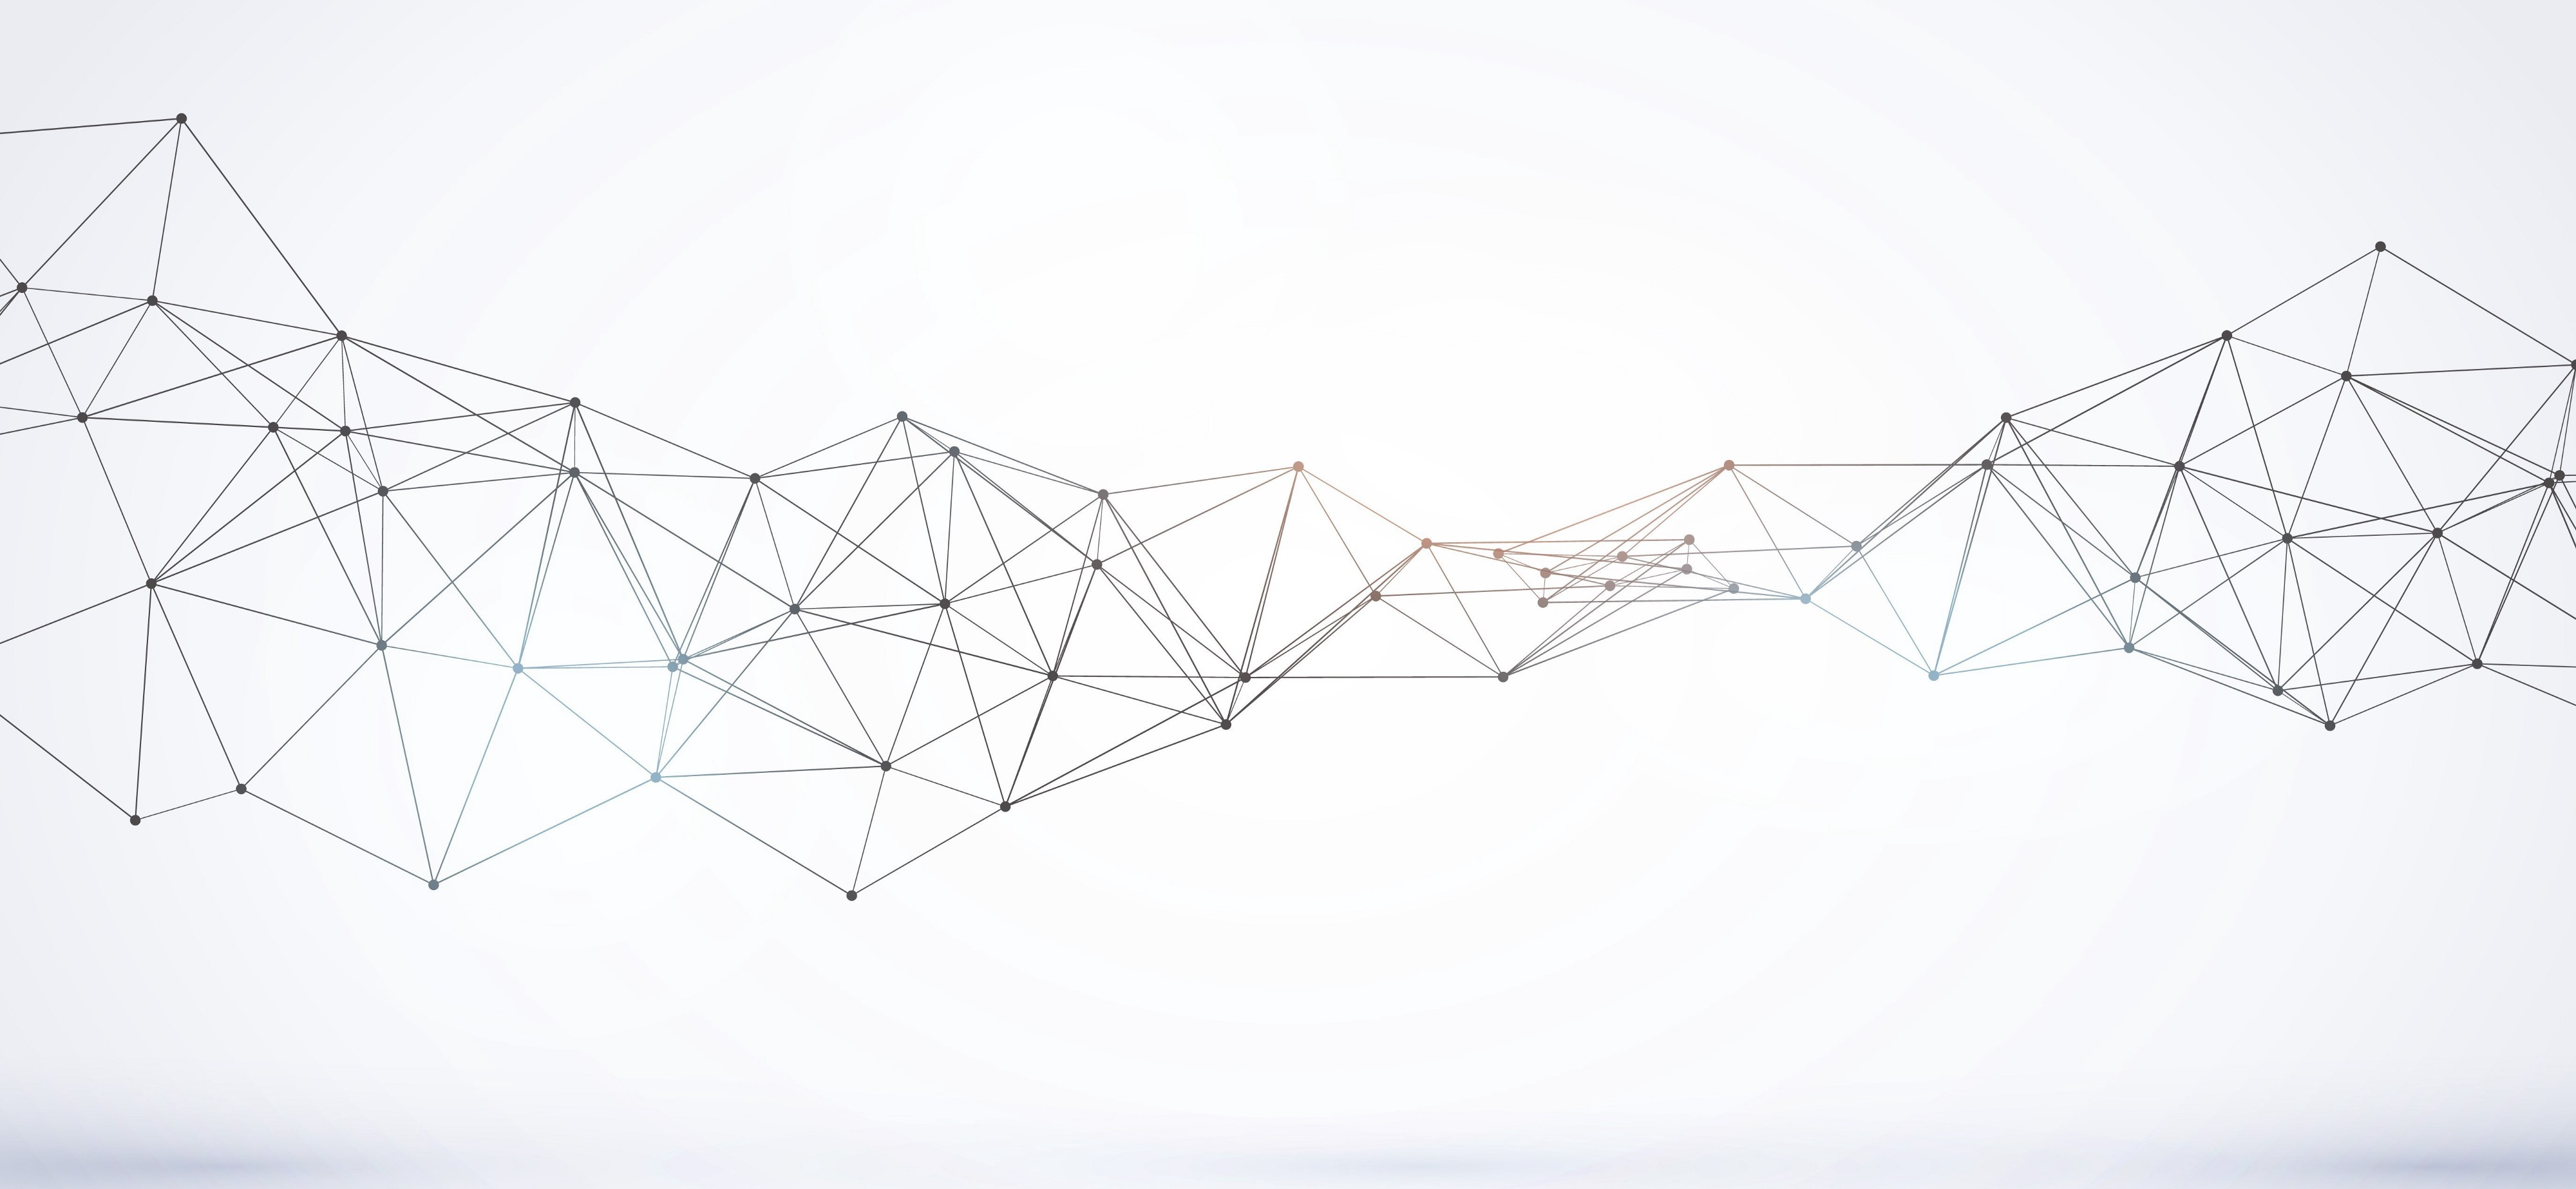
\includegraphics[width=\paperwidth,height=\paperheight]{images/header}};}%
\begin{frame}[plain]
    \vspace{0.5cm}
    \title{\large \begin{spacing}{1.0}Neural Networks for Data Science\end{spacing}\vspace{0.25em}
        \normalsize \begin{spacing}{1.0}\textbf{Master's Degree in Data Science}\end{spacing}\vspace{0.5em}}
    \subtitle{\Large \textbf{Attention and the transformer}}
    \date{
        {
\includegraphics[scale=0.8]{images/Uniroma1}}
    }
    \author{
        \setlength{\tabcolsep}{2pt}
        \begin{tabular}{rl}
            \textbf{Lecturer}: & S. Scardapane \\
        \end{tabular}
    }\titlepage
\end{frame}
}

\part{1}

\section{Designing the transformer}
\subsection{From convolutions to attention}

\begin{frame}{Transformers}
    \setlength{\parskip}{4pt}

    The \myalert{transformer} was proposed in 2017 for machine translation. Like the convolutional models of the
    last lecture, the backbone maps a sequence of embeddings $\vc{X} \sim(T,D)$ to another sequence followed by a task-wise head, e.g.:

    \vspace{0.2em}
    \begin{columns}[T,onlytextwidth]
        \begin{column}{0.48\textwidth}
            \begin{tcolorbox}[nndsblue,courseheight={families}{}]
                \textbf{Sequence classification}\par
                Each output can depend on the whole sequence: we call it an
                \myalert{encoder} transformer (e.g. BERT, ViT).
            \end{tcolorbox}
        \end{column}
        \begin{column}{0.48\textwidth}
            \begin{tcolorbox}[nndsred,courseheight={families}{}]
                \textbf{Next-token prediction}\par
                The model must be causal, as with causal convolutions: we call it a \myalert{decoder} transformer (e.g. GPT).
            \end{tcolorbox}
        \end{column}
    \end{columns}

    \vspace{0.6em}
    As we will see, the original 2017 paper combined both.

    \SlideSource{Vaswani et al. (2017), \href{https://arxiv.org/abs/1706.03762}{\textit{Attention Is All You Need}}, NeurIPS.}

\end{frame}

\begin{frame}{Beyond locality}
    \setlength{\parskip}{6pt}

    A convolution assumes \myalert{locality}: each output mixes a fixed window
    of neighbors. In text, audio or graphs, dependencies can instead be
    \myalert{long-range}, \myalert{sparse} and \myalert{dynamic}.

    Compare:
    \begin{itemize}
        \item \textit{the {\color{darkcerulean}\textbf{cat}} is on the {\color{darkgreen}\textbf{table}}};
        \item \textit{the {\color{darkcerulean}\textbf{cat}}, which belonged to my mother, is on the {\color{darkgreen}\textbf{table}}}.
    \end{itemize}
    The relation between the two words is the same, but their distance is not.

    Stacking layers (or dilating them) grows the receptive field. However, the
    weight given to a neighbor still depends only on its \textit{offset}, never on
    what the two tokens contain.

\end{frame}

\begin{frame}{Convolutions as a sum over offsets}
    \setlength{\parskip}{6pt}

    Take a sequence $\vc{X}\sim(T,D)$ with rows $\vc{x}_t=\idx{\vc{X}}{t,:}$. Because
    transformers come from NLP, we call each row a \myalert{token} and $D$ the
    \myalert{embedding dimension}.

    Ignoring padding and the activation, a 1D convolution with kernel size
    $s=2k+1$ is:
    \[
        \vc{h}_t=\sum_{j=-k}^{k}\eqnmarkbox[drawblue]{wconv}{\idx{\vc{W}}{j+k,:,:}}\,\vc{x}_{t+j}\,,
        \qquad \vc{W}\sim(s,D,D).
    \]
    \annotate[yshift=-0.8em]{below,right}{wconv}{one matrix per offset}
    \vspace{0.6em}

    This is the layer of the CNN lecture, with the kernel reshaped into one
    $D\times D$ matrix for each offset $j$, stored at position $j+k$. Its parameters grow linearly with
    $s$. We want to remove the locality assumption while keeping the number of
    parameters independent of the length $T$.

\end{frame}

\begin{frame}{Continuous convolutions}
    \setlength{\parskip}{6pt}

    Instead of storing one matrix per offset, we \textit{compute} it with a small
    trainable network $g:\mathbb{Z}\rightarrow\mathbb{R}^{D\times D}$ that takes
    the offset as input:
    \[
        \vc{h}_t=\sum_{t'=0}^{T-1}\eqnmarkbox[drawblue]{wcont}{g(t'-t)}\,\vc{x}_{t'}\,.
    \]
    \annotate[yshift=-0.8em]{below,right}{wcont}{weight computed from the offset}
    \vspace{0.6em}

    The kernel now covers the whole sequence with a fixed number of
    parameters. These \myalert{continuous convolutions} also handle inputs of
    variable size and resolution.

    \SlideSource{Romero et al. (2022), \href{https://arxiv.org/abs/2206.03398}{\textit{Towards a General Purpose CNN for Long Range Dependencies in $N$D}}, arXiv.}

\end{frame}

\begin{frame}{Non-local networks}
    \setlength{\parskip}{6pt}

    A continuous convolution handles long-range dependencies, but they are
    still \textit{regular}: the weight depends only on the offset $t'-t$. We
    can let it depend on the \textit{values} of the tokens instead:
    \[
        \vc{h}_t=\sum_{t'=0}^{T-1}\eqnmarkbox[drawblue]{wnl}{\alpha(\vc{x}_t,\vc{x}_{t'})}\,\vc{x}_{t'}\,.
    \]
    \annotate[yshift=-0.8em]{below,right}{wnl}{weight computed from the two tokens}
    \vspace{0.6em}

    This is a \myalert{non-local neural network}. With a suitable choice of
    the weighting function $\alpha$, we will obtain the attention layer.$^1$

    \vfill
    {\footnotesize\color{black!60} $^1$ We could also combine the two ideas, with a
    weight $\alpha(\vc{x}_t,\vc{x}_{t'},t'-t)$ that depends on both the tokens and
    their offset. We will return to this with \textit{relative positional
    embeddings}.\par}

    \SlideSource{Wang et al. (2018), \href{https://arxiv.org/abs/1711.07971}{\textit{Non-local Neural Networks}}, CVPR.}

\end{frame}

\begin{whiteframe}{Three ways to weight a neighbor}
    \setlength{\abovecaptionskip}{6pt}

    \vspace{1em}
    \begin{figure}
        \centering
        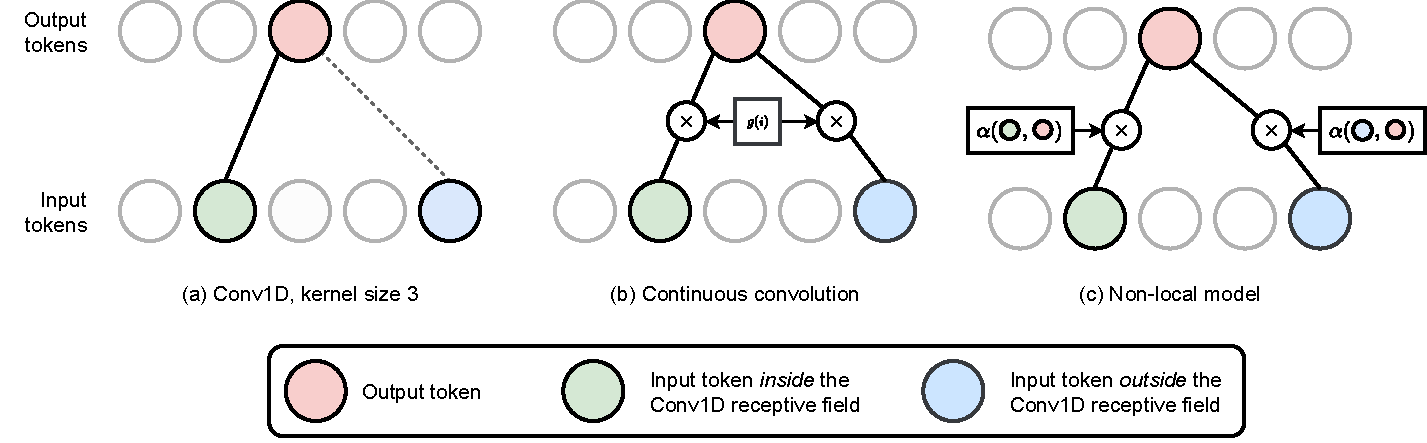
\includegraphics[width=\linewidth]{images/transformers/book/convolution_types.pdf}
        \caption{(a) A convolution with kernel size $3$ has a weight for the
            green token and none for the blue one. (b) A continuous convolution
            weights both with $g$ of their offset. (c) A non-local model
            weights both by their similarity with the token at the output
            position.}
    \end{figure}

\end{whiteframe}

\end{document}
